% !TeX TXS-program:bibliography = txs:///bibtex
%BEGIN_FOLD
\documentclass{article}


%\usepackage[T1]{fontenc}
%\usepackage{svg}
\usepackage[margin=1in]{geometry}
\usepackage{parskip}
\usepackage{bbm}
\usepackage{booktabs}
\usepackage[format=plain,
            labelfont={sl},
            textfont={it,small}]{caption}
\usepackage{tikz}
	\usetikzlibrary{arrows,positioning, cd, calc,shapes.geometric}
	\tikzset{dpadded/.style={rounded corners=5, inner sep=0.7em, draw, outer sep=0.3em, fill={black!50}, fill opacity=0.08, text opacity=1}}
    \tikzset{light pad/.style={outer sep=0.2em, inner sep=0.5em, draw=gray!50}}
	\tikzset{arr/.style={draw, ->, thick, shorten <=2pt, shorten >=2pt}}
    \tikzset{center base/.style={baseline={([yshift=-.8ex]current bounding box.center)}}}
	\tikzset{square/.style={regular polygon,regular polygon sides=4}}

	\newcommand\cmergearr[4]{
		\draw[arr,-] (#1) -- (#4) -- (#2);
		\draw[arr, shorten <=0] (#4) -- (#3);
	}
	\newcommand\mergearr[3]{
		\coordinate (center-#1#2#3) at (barycentric cs:#1=1,#2=1,#3=1.2);
		\cmergearr{#1}{#2}{#3}{center-#1#2#3}
	}
    
\usepackage{mathtools,amssymb}
\usepackage{amsthm}
\usepackage{thmtools} % asmsymb must be loaded also.

	\newtheorem{poss}{Possible Result}
	\declaretheorem[name=Intuition]{intu}
	\theoremstyle{definition}
    \definecolor{defncolor}{rgb}{0.3,0.2,0.5}
	\declaretheorem[name=Definition,qed=$\square$
%		, preheadhook = \color{defncolor}
		]{defn}
	\declaretheorem[name=Def,unnumbered,qed=$\square$,preheadhook = \color{defncolor}]{defn*}
	\declaretheorem[name=Example,qed=$\square$]{example}
	\theoremstyle{remark}
	\newtheorem*{remark}{Remark}
	
\usepackage{color}

\definecolor{deepgreen}{rgb}{0,0.5,0}
\usepackage{hyperref}
\hypersetup{colorlinks=true, linkcolor=blue!50!black, urlcolor=magenta!70!black, citecolor=deepgreen}

\usepackage{framed}

\usepackage{array} 
%\newcolumntype{L}{>{\text\begingroup}l<{\endgroup}} % math-mode version of "l" column type
\newcolumntype{L}{>{$\texttt{/\!\!/ }}l<{$}}

\makeatletter
\renewcommand\@makefntext[1]{%
	\parindent 1em%
	\noindent
	\color{gray}%                        % <----
	\hb@xt@1.8em{\hss\@makefnmark}#1}
\makeatother

\newcommand{\thickD}{I\mkern-8muD}
\DeclarePairedDelimiterX{\infdivx}[2]{(}{)}{#1\;\delimsize\|\;#2}
\newcommand{\kldiv}{\thickD\infdivx}

\newcommand\mat[1]{\mathbf{#1}}


\newcommand{\ed}[3]{#2
	\overset{\smash{\mskip-5mu\raisebox{-4.2pt}{\scalebox{0.6}{$#1$}}}}{\raisebox{-0.5pt}{$\xrightarrow{\hphantom{\scalebox{0.6}{$#1$}}}$}} #3} 

\DeclarePairedDelimiterX{\bbr}[1]{[}{]}{\mspace{-3.5mu}\delimsize[#1\delimsize]\mspace{-3.5mu}}
\DeclareMathAlphabet{\mathdcal}{U}{dutchcal}{m}{n}
\DeclareMathAlphabet{\mathbdcal}{U}{dutchcal}{b}{n}

\newcommand\Set{\mathbb{S}\mathrm{et}}
\newcommand\two{\mathbbm 2}

\newcommand{\D}{\mathbdcal D}
\newcommand{\Attrs}{\mathcal J}
\newcommand{\Idx}{\mathcal I}
\newcommand{\arity}{\mathit{ar}}


\newcommand{\Doms}{{\mathcal D}}
\newcommand{\Rels}{{\mathcal R}}
\newcommand{\sch}{\mathdcal S}%{\sigma}

\newcommand{\bp}[1][L]{\mat{p}_{\!_{#1}\!}}
\newcommand{\V}{\mathcal V}
\newcommand{\N}{\mathcal N}
\newcommand{\Ed}{\mathcal E}


\newcommand{\dg}[1]{\mathbdcal{#1}}
\newcommand{\var}[1]{\mathsf{#1}}
\newcommand{\PDGof}[1]{{\dg M}_{#1}}
\newcommand{\pdgvars}[1][]{(\N#1, \Ed#1, \V#1, \mat p#1, \beta#1)}

\usepackage{enumitem}
\usepackage{float}
\usepackage[noabbrev,nameinlink]{cleveref}

\crefname{example}{example}{examples}
\crefname{defn}{definition}{definitions}
\crefname{prop}{proposition}{propositions}
\crefname{constr}{construction}{constructions}
\crefname{fact}{fact}{facts}

\usepackage{subcaption}
	\captionsetup[subfigure]{subrefformat=simple,labelformat=simple}
	\renewcommand\thesubfigure{(\alph{subfigure})}

\newlength\todolength
\setlength\todolength{\textwidth-5pt}
\newcommand{\todo}[1]{
%\textbf{$\smash{\Large\boldsymbol{[}}$
		\colorbox{red!60!black}{\parbox{\todolength}{\color{white}$\mathrlap{\textbf{todo}}${\hspace{0.12ex}}\textbf{todo}: #1}}
%	 \!\!\smash{$\Large\boldsymbol{]}$}\!}
}


%END_FOLD

\begin{document}
\begin{center}
  \textbf{ \Large Databases:} how relational databases are deterministic PDGs,\\
  and the of using PDG semantics to emulate databases.
\end{center}

% \section*{Layout Of This Document}
% \begin{description}
%     \item[\textbf{The World of Deterministic Databases}] Definitions
% \end{description}
\section{Motivation and Overview}

A probabilistic databases are known to be related to graphical models \cite[\S 1.2.7]{suciu2011probabilistic}. Specifically, a probabilistic 

As far as the graphical model community is concerned (see Chapter 6 of \cite{KF09} for an overview), the right way to model higher order information such as indexed collections of variables, is to create a ``template'' graphical model, which can be compiled to a ground-level model, and then acts as usual. There many ways to do this, but emperically the most popular one is the \emph{plate model}, illustrated by their prevalence on the wikipedia articles for common families of statistical models (\Cref{fig:platemodel-ex})
and in probabilistic programming frameworks, such as \href{https://pyro.ai/}{Pyro}'s \href{http://docs.pyro.ai/en/0.3.0-release/primitives.html#pyro.plate}{plate constructor}.

\begin{figure}[H]
	\centering
	\hfill%
	 \raisebox{-0.5\height}{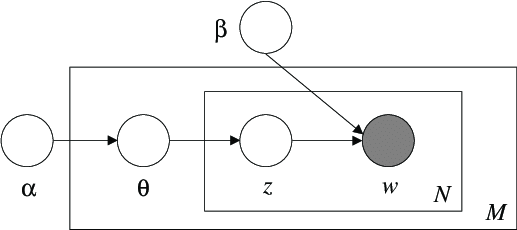
\includegraphics[width=0.3\textwidth]{img/lda.png}}%
%	\hfill\vline\hfill%
	\hfill%
	 \raisebox{-0.5\height}{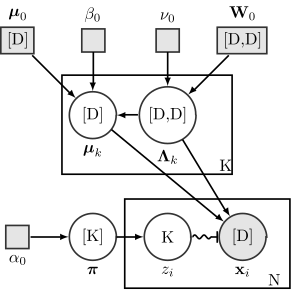
\includegraphics[width=0.3\textwidth]{img/gaussian-mixture-switch.png}}%
	\hfill~\\
	\caption{Plate Models from the Wikipedia pages for \href{https://en.wikipedia.org/wiki/Latent_Dirichlet_allocation}{LDA} and  \href{https://en.wikipedia.org/wiki/Mixture_model}{Gaussian Mixture Model}.%
			\protect\footnotemark
		}\label{fig:platemodel-ex}

\end{figure}
% Now, the text of the footnote from the figure
\footnotetext{{Note that the formal presentation of plate models given in \cite{KF09} is not as expressive as the their usage in the wild; for instance, the Gaussian mixture model on the right has arrows leaving a plate, which is forbidden by \cite{KF09}.}}




On the other hand, many 



\begin{description}
	\item[The problem I'm solving.]
	\item[Why this problem is intereesting.]
	\item[Some example instances of the problem.]
	\item[Why this problem is non-trivial.]
\end{description}


%
%\subsection{Ways of Probabilizing}
%\begin{enumerate}
%	\item 
%\end{enumerate}

%\section{Background: Databases, PGMs, and First-order Uncertainty}

\section{Deterministic Databases}

There are several equivalent ways of thinking of a database. Due to the correspondence to first-order predicates and their logics, it is often theoretically convenient to think of databases relationally. This has also been argued \cite{Codd} to be a more natural, access-path-independent representation of the data.   

Recall Vardi's \cite{vardi} definition of a relational database:
\begin{leftbar}	
\begin{defn*}
    An (untyped) database is a tuple $(D, R_1, \ldots, R_k)$, where $D$ is a finite set, and for each $i$, we have $R_i \subseteq D^{a_i} = \prod_{j =1}^{a_i} D$ 
    %(equivalently to emphasize structural similarity with the definition below, $R_i \in 2^{D^{a_i}}$)
    for some \emph{arity} $a_i \in \mathbb N$. 
\end{defn*}
\end{leftbar}

We alter the presentation and notation slightly, without changing the mathematical structure, so that can formally define $a$, and avoid possible future confusion with the numbered indices. 

\begin{defn}[untyped relational database]
    An untyped relational database is a tuple $(D, I, \arity, \mathcal R)$, where $D$ is a
    finite set (the universal domain), $I$ is a finite index set, $\arity: I \to
    \mathbb N$ is the arity function (for each $i \in I$, $\arity_i$ is the
    \emph{arity} of the $i^{\text{th}}$ relation), and $\mathcal R = \{R_i\}_{i
    \in I}$ is a finite collection of relations on $D$, so that for each $i \in
    I$, we have $R_i \subseteq D^{\arity_i} = \prod_{j =1}^{\arity_i} D$.
\end{defn}

Though theoretically simple, this presentation requires a  ``universal domain'' $D$, whose meaning can be muddled. This can have annoying practical consequences; for instance, a government database of inhabitants might include a unary predicate $\texttt{isCitizen}$, intended for people, but also a binary predicate \texttt{isCauseOfDeath} for people and diseases. If we use a single domain, we must specify whether or not each cause of death is also a citizen; one might be happier with a type error.
It is also common to insist that attribute names are always distinct, and as a pragmatic matter, the diagrams here will be much less convincing. 
%
We are therefore more interested in a \emph{typed} definition of a database, of which the previous definition is a special case.

\begin{defn}%[database]
    A (typed) database $\D$ is a tuple $\D = (\Attrs, \Idx, \Doms, \sch, \Rels)$, where
    
    
        \def\oftype#1{{$:#1$}}
    
    \renewcommand{\arraystretch}{1.3}
    \begin{tabular}{@{~~~}r@{}lp{13cm}}
    	$\Attrs$ & \oftype{\Set} & is a finite set of attribute names, \\
    	$\Idx$ & \oftype{\Set} & is a finite set of table names,\\
    	$\Doms$ & \oftype{\Attrs \to \Set} & assigns a domain of possible values to each attribute name, and \\
    	$\sch$ & \oftype{\Idx \to \Attrs \to \two,} & called the \emph{schema} of $\D$, assigns a multi-set of attribute names $\Attrs$ to each table name (corresponding to the table columns).
 \\[0.5em]\multicolumn{3}{@{}p{\textwidth}@{}}{
 	In this way, $\sch$ gives the database type structure: it ensures that column $j$ of the $i^\text{th}$ table comes from the specific attribute $j \in \Attrs$. The arity function can be defined by flattening all of the type information in the schema, and reducing $\sch_i$ to its length: $\arity(i) := | \sch_i |$.
	Together, $\sch$ and $\Doms$ determine a product domain $\mat D_i := \prod_{j \in \sch_i} \Doms_{j}$ of valid tuples in the relation $R_i$. With this, we can define the final and most important component of a database, the tables themselves:
		} \\
%    	 \rule{0pt}{1.3\normalbaselineskip} $\Rels$ & \oftype{(i:\Idx) \to \prod_{j \in \sch_i} \Doms_{j} \to 2}&
    	 \rule{0pt}{1.3\normalbaselineskip} $\Rels$ & \oftype{(i:\Idx) \to \mat D_i \to \two}&
    	is an $\Idx$-indexed collection $ \{ R_i \}_{i \in \Idx}$ of relations, where each $R_i \subseteq \mat D_i$.
    \end{tabular}
    
%    \def\oftype#1{{\!\!$:#1\qquad$}}
%    \begin{itemize}[itemsep=-0.8ex]
%    	\item[$\Attrs$] \oftype{\Set} 
%    		is a finite set of attribute names.
%    	\item[$\Doms$] \oftype{\Attrs \to \Set} 
%    		assigns a set of possible values to each attribute name.
%    	\item[$\Idx$] \oftype{\Set} 
%    		is a finite set of table names.
%%    	\item[$\arity$] \oftype{\Idx \to \mathbb N} 
%%    		is the arity function, so that $\arity(i)$ is the number of columns in the $i^\text{th}$ table.
%    	\item[$\sch$] \oftype{\Idx \to \Attrs \to 2,}
%    		%\oftype{\Idx \to \{1, \ldots, \arity(i)\} \to  N,}
%    		called the \emph{schema} of $\D$, gives the database type structure by ensuring that the $j^\text{th}$ column ($j < \arity(i)$) of the $i^\text{th}$ table comes from the specific attribute $\sch_{i,j} \in \Attrs$. 
%    \end{itemize}
    
%    $\mathcal D$ is a collection of finite domains (the domain for each attribute), 
%	again $\arity: I \to \mathbb N$ determines the arity of , but now 
	
%	For $i \in I$ and $j \in \{1, \ldots, \arity(i)\}$, we write $A_{i,j}$ for the $j^{\text{th}}$ component of the relation $R_i$, so that the relation $R_i$ 
	
%	Once again $\mathcal R =$ is a finite collection of relations, though now their types are determined by $\Att$. Let 
%	$$\mat D_{i} :=  \prod \Att_i = \prod_{j =1}^{\arity(i)} \Att_{i,j}$$
%	be the possible tuples that could 
	
%	$R_i \subseteq \prod \Att_i = \prod_{j =1}^{\arity(i)} \Att_{i,j} $
	\smallskip	
	Since $\Idx$, and $\Attrs$ are implicit in the type of $\sch$, and $\Doms$ is implicit in the definition of $\Rels$,
	we sometimes use the abbreviated form $\D = (\sch, \Rels)$. %where $\sch$ is understood to be packaged with appropriate data for $\Idx, \Attrs$, and $\arity$. 
\end{defn}
%\begin{defn}
%	The component $\Att^\D$ of a typed database $\D = (\mathcal D, I, \arity, \Att, \mathcal R)$, is the \emph{schema} of $\D$. %$(I, \Att)$ defines a hypergraph. 
%\end{defn}

%\begin{remark}
%	$(I, \Att)$ is a hyper-graph, and $D$ assigns 
%\end{remark}

\begin{remark}\label{rem:typed-db-better}
    The definition of an untyped database with underlying domain $D$ is a special case of a typed database, where $\Attrs = \mathbb N$ corresponding to the argument index, set every $\Doms_n := D $, and every $\sch_{i,j} = \mathbbm1[j \le \arity(i)]$. 
    In some sense, the two are equally expressive: we can also simulate a typed database $\D$ with an untyped one. Simply set $D := \uplus_j \mathcal D_j$ to be the disjoint union of all domains, and $\arity(i) := |\sch_i|$. Now any table $R_i \in \Rels^\D$ can be directly used as a table in the untyped database, since
    \[R_i \subseteq \mat D_i = \prod_{j \in \sch_i} \mathcal D_{j} 
		\subseteq \prod_{j \in \sch_i} D = \prod_{j = 1}^{\arity_i} D = 
        D^{\arity(i)} .\] 
  	The definitions are not equivalent, and the typed version is more expressive, because it disallows some rows by fiat (which has a different meaning from being absent from the relation), encoding type-level constraints. This is nice even within the context of databases, since a ds. By naming $A$, we can explicitly restrict the  allowable collections of attributes, which with which we will be able to define classes of databases which behave like other specific graphical models.
\end{remark}

\begin{example}\label{ex:abcd}
	Consider a database $\D$ with three tables $R_1, R_2, R_3$, where $R_1$ has columns $\{A,B,C\}$, $R_2$ has columns $\{B,D\}$, and $R_3$ has columns $\{C,D\}$. The data we have specified so far is qualitative in nature, and forms precisely the schema.
	%(and the other components of a typed database implicit in it).
	Formally, it is given by
	\[ 
	\begin{array}{c}
		\Idx = \{1,2,3\};\\
		\Attrs = \{A,B,C,D\};
	\end{array}
	\quad
%		\arity = \left[\begin{array}{cc}
%			1 &\mapsto 3 \\ 2 &\mapsto 2 \\ 3 &\mapsto 2
%		\end{array}\right];	\quad
		\sch = \left[\begin{array}{rl}
				1 &\mapsto \{A, B, C\} \\
				2 &\mapsto \{ B, D \} \\
				3 &\mapsto \{C, D\}
			\end{array}\right]
%	 \sch_1 = \{A, B, C\};\quad \sch_2 = \{ B, D \};\quad \sch_3 = \{ C, D \}, 
\] 
	as depicted in \Cref{fig:sketches}.
\end{example}

We now begin the further classification of databases, by their schemas, as mentioned in \Cref{rem:typed-db-better}.  
By considering databases that have a specific kind of schema $\sch$, we will effectively requiring topological properties of the corresponding PDG, which will clarify the kinds of complexities involved with querying. Specifically, we consider restrictions to database schemas $\sch$ for which:


\begin{enumerate}[nosep, label={\textbf{Class \arabic*:}},ref={class \arabic*}]

	\item % graph is disconnected (cell independence) 
		\textit{Every attribute is globally unique.}
		This occurs iff $\sch$, viewed in uncurried form as a function $\sch : I \times \to \Attrs$, is injective. 
		In the absence of any other information, such databases are not particularly interesting, because no table any relationship to any other, and one may as well consider them separately. We will see in \Cref{sec:usage-of-of-disjoint-table} that this class of database can still be useful if we add additional nodes and links to the resulting PDG.
		\label{class:guniq}
				
	\item % graph is bipartite. 
		% paths are zig-zags.
		\textit{Each attribute of a table is unique.}
		If $\sch$ has a weaker property, namely that each $\sch : [\arity(i)] \to \Attrs$ is a injective, then each local table looks like a component of a larger map, where the cuts happen along attributes $\sch$. The alignment of the values of $\sch$ suggest a ``gluing'' of tables together. This corresponds to a natural join. 
		\label{class:luniq}
%	\item 
%	chordal graph is impossible.
	\item \textit{No restrictions on $\sch$.} The difference between this class and the previous one is the possibility of self-joins. Self-joins \cite{DS04}.
		\label{class:nuniq}
\end{enumerate}

	The different classes can be converted two and from one anther. A \ref{class:guniq} schemas.
	
\subsection{Warmup: Databases and Constraint Graphs}

Consider again \Cref{ex:abcd}, and in particular its depiction in the center of \Cref{fig:sketches}, which is an undirected hyper-graph; it looks exactly like a graphical depiction of a factor graph on the variables $\{A,B,C,D\}$. Moreover, there is an obvious choice of factor --- just evaluate the relation as a function from its argument domains to $\{0,1\}$. For instance, given a tuple $(a,b,c)$, the factor corresponding to the relation is
 
\[ \phi_1( a,b,c) := \mathbbm1[(a,b,c) \in R_1]=  \begin{cases}
	+1 & \text{if } (a,b,c) \in R_1 \\ 0 & \text{otherwise}
\end{cases}
\]
 
 
%\[ \phi_1(a,b,c) := \mathbbm1[(a,b,c) \in R_1]=  \begin{cases}
%	+1 & \text{if } (a,b,c) \in R_1 \\ 0 & \text{otherwise}
%\end{cases}
%;\qquad 
%\phi_2(b,d) := \begin{cases}
%	+1 & \text{if } (b,d) \in R_2 \\ 0 & \text{otherwise}
%\end{cases}. \]
In this sense, the resulting constraint graph%
\footnote{a constraint graph is the specific factor graph where each factor is binary.
	Interpreted with factor graph semantics, it gives the uniform distribution over joint settings that satisfy the constraints, because each world either has a score of 1 or 0, and the result is normalized.}
respresents a set of complete choices of domain elements $(a,b,c,d)$ that satisfies all three relations (that is, $(a,b,c) \in R_1$, $(b,d) \in R_2$, and $(c,d) \in R_3$), which in this case consists only of $\{(a_2,b_2, c_2,d_1)\}$. If there were no overlap between the values of $B$ in the two tables, the constraints would be unsatisfiable. 

For the analogy to make sense, implicitly, a ``possible world'' is in this setting must be a selection from each domain.
This is of course not at all what most people would mean say about a ``possible world'' in the setting of probabilistic databases. 
The dominant view is that a particular database is a constraint graph, and so a probabilistic database is a distribution over constraint graphs. 

 in which a possible world is a complete database, and the tables on the left of \Cref{fig:sketches}. Specifically, we will need to address the following issues with this picture:

\begin{enumerate}
	\item  In general, we are not thinking of  $A, B, C, D$ as random variables that ``take a single value''; all attributes are taken at once by different elements of the domain. We will argue why that this practice is not meaningfully different from what needs to be done to model other things with graphical models; we will ultimately resolve it in a more satisfactory way in \Cref{sec:possible-world}.
	\item Even if there is a reasonable notion of ``possible world'' that is a joint setting of attributes, the mere existence of a table in a database does not constitute an assertion that its corresponding relational predicate is true. In fact, any table with zero rows (an empty relation) is unsatisfiable, making the corresponding graphical model inconsistent. This is resolved by conditioning on the truth of the predicate itself (which we call a \emph{link guard}) in \Cref{sec:link-gurad}. This turns out to be equivalent to adopting the stance that some variables can take a ``none of the above'' value, on which interpretations of arrows are silent%
	\footnote{This is the left half of the additional benefit we get from general PDGs over strict ones; the right half is not assigning all of the probability mass, or \emph{sub-stochasticity}. }
\end{enumerate}

\section{Database Schemas and Qualitative PDGs}

We will divide database schemes into classes complexity



First, we show how to encode a database in a PDG. There are multiple ways to structure a database; even with the tools of a relational database, it is possible to encode data in multiple ways, some of which are more ``relational'' in nature, and others which are more path dependent, and are perhaps better thought of as an object graph. 
Before we get into the details (\Cref{sec:PDG-db-details}), we'll start with some illustrations. 


\subsection{Illustrations}


\begin{figure}
    \centering
    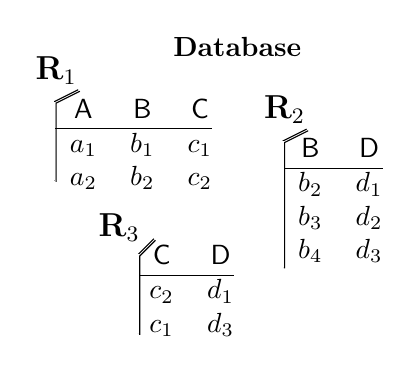
\begin{tikzpicture}[baseline=0, tablename/.style={inner sep=1pt,circle,text=black,font={}}]
    	 %fill=gray!20
        \node at (1,1.5){\textbf{Database}};
               
        \node[tablename] (R1) at (-1.3,1.2) {\large$\mathbf R_1$};
        \node[below right=-0.2em and -1.2em of R1] (table1) {
            \begin{tabular}{ccc@{}}
                $\var A$ & $\var B$ & $\var C$\\\hline
                $a_1$ & $b_1$ & $c_1$ \\ $a_2$ & $b_2$ & $c_2$ 
            \end{tabular}
        };
	    \draw[] ($(R1.south)+(.3,.1)$) -- ++(-0.3,-0.15) -- ++(0,-1);
  		\draw[] ($(R1.south)+(.28,.12)$) -- ++(-0.3,-0.15) -- ++(0,-1);
  		\fill[white] ($(R1.south)+(.29,.12)+(-0.3,-0.15)$) rectangle ++(-0.1,-1);
  		
  		
  		\node[tablename] (R3) at (-0.5,-0.8) {\large$\mathbf R_3$};
  		\node[below right=-0.6em and -0.6em of R3] (table1) {
  			\begin{tabular}{cc@{}}
  				$\var C$ & $\var D$\\\hline
  				$c_2$ & $d_1$ \\ $c_1$ & $d_3$  
  			\end{tabular}
  		};
  		\draw[] ($(R3.south east)+(.2,.1)$) -- ++(-0.2,-0.2) -- ++(0,-1);
  		\draw[] ($(R3.south east)+(.18,.12)$) -- ++(-0.2,-0.2) -- ++(0,-1);
  		\fill[white] ($(R3.south east)+(.19,.12)+(-0.2,-0.2)$) rectangle ++(-0.1,-1);
    
%        \node[draw,circle,inner sep=0.2pt,fill=gray!50] (R2) at (1.3,1) {\large$R\mspace{-3.5mu}R_2$};
        \node[tablename] (R2) at (1.6,0.7) {\large$\mathbf R_2$};%\mspace{-12.5mu}R
        \node[below right=-0.2em and -1.2em of R2] (table2) {
            \begin{tabular}{cc@{}}
                $\var B$ & $\var D$ \\\hline
                $b_2$ & $d_1$ \\ $b_3$ & $d_2$ \\
                $b_4$ & $d_3$
            \end{tabular}
        };
	    \draw[] ($(R2.south)+(.3,.1)$) -- ++(-0.3,-0.15) -- ++(0,-1.6);
	    \draw[] ($(R2.south)+(.28,.12)$) -- ++(-0.3,-0.15) -- ++(0,-1.6);
	    \fill[white] ($(R2.south)+(.29,.12)+(-0.3,-0.15)$) rectangle ++(-0.1,-1.6);
    \end{tikzpicture}
    \hfill\vline\hfill
    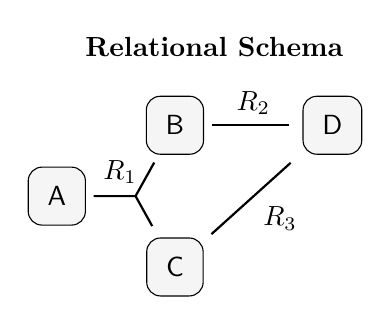
\begin{tikzpicture}[baseline=0]
        \node at (0,1.5) {\textbf{Relational Schema}};
        \node[dpadded] (A) at (-2,-0.4){$\var A$};
        \node[dpadded] (B) at (-0.5, 0.5){$\var B$};
        \node[dpadded] (C) at (-0.5,-1.3){$\var C$};
        \node[dpadded] (D) at (1.5,0.5){$\var D$};

        \coordinate (ABC) at (barycentric cs:A=1,B=1,C=1);
        \node[above left=1pt and -4pt of ABC]{$R_1$};
        
        \draw[arr, -, shorten >=0, shorten <=1.5pt] (A) -- (ABC) (B) -- (ABC) (C) -- (ABC);
        \draw[arr, -, shorten >=0] (D) -- node[above]{$R_2$} (B);
        
	    \draw[arr, -, shorten >=0] (D) -- node[below right]{$R_3$} (C);
    \end{tikzpicture}
    \hfill\vline\hfill
    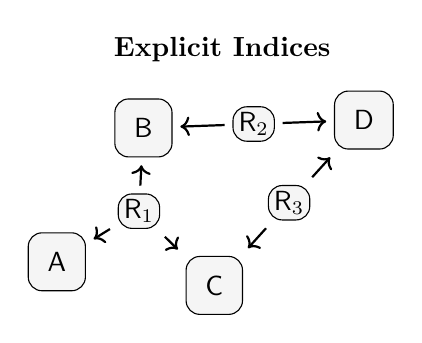
\begin{tikzpicture}[baseline=0]
        \node at (1.5,1.5) {\textbf{Explicit Indices}};
        \node[dpadded] (A) at (-0.6,-1.2){$\var A$};
        \node[dpadded] (C) at (1.4,-1.5){$\var C$};
        \node[dpadded] (B) at (0.5, 0.5){$\var B$};
        \node[dpadded] (D) at (3.3,0.6){$\var D$};

        \node[dpadded,inner sep=2pt] (R1) at (barycentric cs:A=1,B=1.5,C=1){$\var R_1$};
        \node[dpadded,inner sep=2pt] (R2) at (barycentric cs:B=1,D=1){$\var R_2$};
        \node[dpadded,inner sep=2pt] (R3) at (barycentric cs:C=1,D=1){$\var R_3$};
        % \node[above left=1pt and -4pt of ABC]{$R_1$};
        
        \begin{scope}[->, thick, shorten <=0pt, shorten >=0pt]
            \draw (R1) -- (A);
            \draw (R1) -- (B);
            \draw (R1) -- (C);
            \draw (R2) -- (B);
            \draw (R2) -- (D);
            \draw (R3) -- (D);
            \draw (R3) -- (C);
        \end{scope}
    \end{tikzpicture}
    
    \caption{a simple relational database (left), the undirected hyper-graph depicting its schema (center), and an encoding as a PDG including variables for the row indices (right). Note that we must interpret the two rows into B separately, and not as a joint dependence, so the directed representation is not possible with standard graphical models.} \label{fig:sketches}
\end{figure}
\begin{example}
    With reference to \Cref{fig:sketches}, let's construct a typed relational database with domains $\var{A, B, C, D}$, and relations $R_1 \subseteq \mathcal V(\var{A\times B \times C}); R_2 \subseteq \mathcal V(\var{B, D})$. To specify $R_1$ and $R_2$ is to fill in rows of the tables on the left of the figure. We then present two graphical illustrations.
    
    \textit{The Left, Undirected Diagram.}

    

    
    % By representing $f$ in un-curried form, we only need to solve the second
    % problem. Specifically, suppose we indeed wanted to assert the truth of each
    % predicate. A relation is defined by the set of tupples it contains, and
    % because the constraint graph gives a set of admissible tuples, the resulting
    % set of joint settings is the set of

    
    \textit{The Right, Directed Diagram.} On the far right of \Cref{fig:sketches}, we have an a directed presentation, employing roughly the same trick we used to present PDGs as graphs rather than hyper-graphs. This is the object that can naturally be encoded as a PDG, and is the picture we will be defending. More concretely, the change is to create new index variables $R_1$ and $R_2$, for the rows of the database. 
    
    This should feel slightly uncomfortable. One reason for discomfort is the same as the reason we were uncomfortable with writing the attributes $\var{A,B,C,D}$ as variables in the first place (all attributes are likely actualized); a second is the fact that rows in a table and attributes are different kinds of things. The query language allows only references to the former. We add them to the diagram anyway.
    A reader--even one wanting to reject the premise that any of this has meaning---should pause at this point and make sure they appreciate the alignment of this last picture with the original tables. Each row of $R_1$ gives a value of $\var{A,B}$, and $\var C$, while each row of $\var R_2$ gives a value of $\var{C}$ and $\var D$. 
    
    As is standard in the definition of a relational databases, the ``variable'' associated to the relation takes values which are tuples of values. A row is identified with tupples of possible values of the columns, which makes the correspondence between $R_1$ and the product node $\var{A \times B \times C}$ particularly stark, but we will often instead have an explicit column for the ``primary key'' of the table, which can just be the row number. Therefore, rather than thinking of $R_1$ as taking a value $(a,b,c)$, we prefer to think of it as just the variable which identifies the row of the database. Doing so will also eliminate some ambiguity when we introduce uncertainty.
    We have suggested it is all possible tuples ($a,b,c$), but in this case the functions are only partial; we can fix this for now by setting $\V(R_1)$ to be only those tuples that are in $R_1$ --- but without also allowing non-strict PDGs, this has the effect of asserting that it is impossible for there to be any other row in the database. Without any changes, any empty table would have the effect of making all worlds infinitely inconsistent --- we'll provide more details on the fix in \Cref{sec:link-gurad}.
        
    Note also that our earlier observation (that rows and columns of relational databases act differently) can also be seen directly in the structure of the graph; the attributes are exclusively arrow targets, while the row number variables are are only sources. Later we will encounter ways in which foreign keys and references change the picture. Relational databases enjoy special properties because they are \emph{bipartite PDGs} --- their underlying multi-graphs form a directed bipartite graph, in which all the arrows are aligned.
    
    % Specifically, rather than talking about the relations $R_1$ and $R_2$, we can refer to the rows of the table. 
    
    %The arrows from the variables representing either relation, to the variables representing associated attributes are clearly given by the tables on the left of \Cref{fig:sketches}.

\end{example}

Next we tackle something that is clearly first-order and relational in nature, and argue that its interpretation as a graphical model is also appropriate.

\begin{example}[\texttt{isFriend}]
    Suppose we have a domain $\var P$ of people, and a relation $xFy$, indicating whether person $x$ is friends with $y$, for $x,y\in \var P$. 
    The natural thing to do in the first-order case is to interpret this predicate $F$ by giving a subset $f \subseteq \var P \times \var P$, or equivalently, a binary matrix $f : \var P^2 \to 2$. 
    In some sense, a selection of such a function the natural notion of ``possible world'' --- by describing the entire matrix you can be sure you've modeled every relevant distinction as a different possible world. The two visualizations of this setup as graphical models are given in \Cref{fig:friendrel}.
    
    \begin{figure}
        \centering
        \hfill
        \begin{subfigure}[]{0.4\textwidth} \centering
            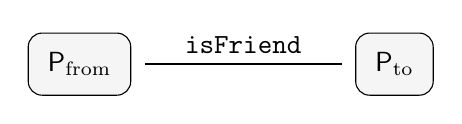
\begin{tikzpicture}[baseline]
                \node[dpadded] (P1) at (-2,0) {$\var P_{\text{from}}$};
                \node[dpadded] (P2) at (2,0) {$\var P_{\text{to}}$};
                
                % \node[] (2) at (0,-1){2};
                % \mergearr{P1}{P2}{2}
                % \node[below=1pt of center-P1P22] {\texttt{isFriend}};
                \draw[arr,-] (P1) -- node[above] {\texttt{isFriend}} (P2);
            \end{tikzpicture}
%            \caption{Lorem ipsum}
        \end{subfigure}
        \hfill\vline\hfill
        \begin{subfigure}[]{0.4\textwidth}\centering
            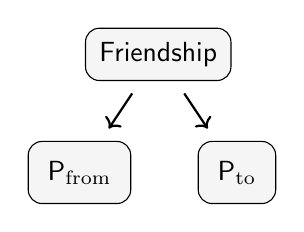
\begin{tikzpicture}[baseline=0]
                \node[dpadded] (P1) at (-1,-0.5) {$\var P_{\text{from}}$};
                \node[dpadded] (P2) at (1,-0.5) {$\var P_{\text{to}}$};
                \node[dpadded, inner sep=5pt] (F) at (0,1) {$\var{Friendship}$};
                
                \draw[arr] (F) to (P1);
                \draw[arr] (F) to (P2);
            \end{tikzpicture}
%            \caption{Lorem ipsum}
        \end{subfigure}
        \hfill
        \caption{}
        \label{fig:friendrel}
    \end{figure}


    For a specific context in which one intends to use the function $f$ in some way, there is also a further ``possible world'' one might have intended: the answers to the queries. As far as an agent is concerned, there is no difference between $f$ and $f'$, so long as $f(p,q) = f'(p,q)$ for every input $(p,q)$ we give it. In other words, the counterfactual information potentially present in $f$, which is not revealed by $f$, need not be modeled as a possible world. For instance, if we imagine a probability system in which we only ask if the particular people Joe and Oli are friends, the rest of the matrix is irrelevant.     
    Moreover, if our language only contains enough symbols to ask this question, the rest of the matrix is irrelevant. 
    The key point is that to ask a question of a PDG, the concept must already exist in the PDG, which dramatically reduces the query language. In turn, this will sometimes allow us us to avoid a full description of the full first-order model of possible worlds. 

    There are also other, more object-y ways of describing the data. In particular we could encode friendship as a probabilistic transition (i.e., weight each friendship, and then normalize), resulting in the following, very simple diagram:
    \begin{center}
        \hspace{1cm}
        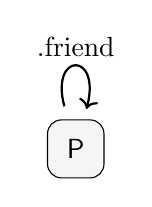
\begin{tikzpicture}[baseline=0]
            \node[dpadded] (P) at (0,0) {$\var P$};
            \draw[arr] (P) edge[loop above] node{.friend} (P);
        \end{tikzpicture}
    \end{center}
    In order for distribution to be consistent with this PDG, it must be a stationary distribution for the Markov Chain generated by the function .friend, which in this case is a simple eigenvalue decomposition of the friend matrix. This examples also suggests tha the notions between our possible worlds can be tied together by unraveling a PDG as a sequence of computations; we give PDGs a more general semantics as an automaton in \Cref{sec:automaton}.
\end{example}


Now we go the reverse direction, and show how graphical models define a database. Here too, both notions of a ``possible world'' ---as either a complete setting of a database, or a joint setting of random variables--- are defensible.
\begin{example}\label{ex:smoking}
    Take the smoking / cancer Bayesian Network, shown below.
    \begin{center}
    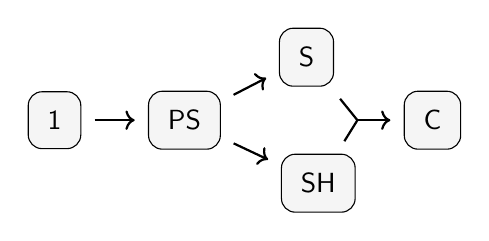
\begin{tikzpicture}
    \node[dpadded] (1) at (0,0) {$\var 1$};
    \node[dpadded] (PS) at (1.65,0) {$\var{PS}$};
    \node[dpadded] (S) at (3.2, 0.8) {$\var S$};
    \node[dpadded] (SH) at (3.35, -0.8) {$\var{SH}$};
    \node[dpadded] (C) at (4.8,0) {$\var C$};
    
    \draw[arr] (1) -- (PS);
    \draw[arr] (PS) -- (S);
    \draw[arr] (PS) -- (SH);
    \mergearr{SH}{S}{C}
    \end{tikzpicture}
    \end{center}
    
    We will start as before with the deterministic case; here this means every arrow is a deterministic function. What is the right notion of a ``possible world''? Is it:

    \begin{enumerate}[label=(\arabic*)]
        \item A setting $ps$ of $\var{PS}$, from which all variables are determined? \label{item:initsetting}
        \item A joint setting $(ps, s, sh, c) \in \V(\var{PS \times SH \times S \times C})$ of all variables? \label{item:jointsetting}
        \item A selection $ps,f,g,h \in \Big(\var{\V(PS) \times \V(S)^{\V(PS)}\times \V(SH)^{\V(PS)}\times \V(C)^{\V(S\times SH)}} \Big)$ of every function? \label{item:everyfunction}
    \end{enumerate}
    
    Again there is more than one reasonable notion. I am not fond of \Cref{item:initsetting}, as I believe it is a mistake to draw a distinction between a setting of $\var{PS}$ (an order 1 tensor, which we have worked hard to expose) and the relationships between other variables (the order 2 and 3 tensors here), but I include the option for future analogy. A treatment in \Cref{item:initsetting}, where the functions do not play any part in the description of the world, is uninteresting; the possible worlds are just the possible values of $\var{PS}$, and if we take the interpretation of $\var 1$ seriously (as we should), there is only one possible world: the unique value $\star$, from which all values are determined. 
    
    By contrast, I argue that both \Cref{item:jointsetting,item:everyfunction} are reasonable. \Cref{item:jointsetting} needs less explanation in this context, in which one is already imagining joint distributions over the four variables. Thus we defend \Cref{item:everyfunction} first.
    We have argued that the arrows themselves must appear in the possible world; after all, the agent is representing beliefs not about the distributions of themselves, but rather how they must interact.
    In \Cref{item:everyfunction}, the function $f: \var{PS} \to \var{SH}$ agent's belief about the relationship between $S$ and $SH$, and the world could well have been such that there was a different relationship between them; therefore in some sense an \emph{complete} description of the world must include these functions also. 
         
    In this deterministic setting, the extra data in \Cref{item:everyfunction} not included in \Cref{item:jointsetting} is the is clearly counter-factual: it describes rules that were never applicable, regarding what \emph{might have} happened, had some other bit of data been set in another way. For instance, the agent believes that the value of $f(ps')$ for $ps' \neq ps$ is totally irrelevant from the outcome (because in fact the agent believes $\var{PS}$ takes the value $ps$, not $ps'$). 
    If we are uncertain about the outcomes and also the functions, but only observe the result of their application, then any data in \Cref{item:everyfunction} but not \Cref{item:jointsetting} cannot be observed; in this sense, it is not part of the outcome. 
\end{example}

\subsection{Attribute Uniqueness}

One reason these examples behave differently is that they have different attributes.

\begin{enumerate}[nosep]
	\item Globally Unique Attributes
	\item Attributes are unique per table
	\item Attributes can be duplicated in a table, with different names.
\end{enumerate}

The last of these can be thought of as a particular way 

\section{What is a World, Anyway?} \label{sec:possible-world}

\begin{example}\label{ex:student}
    There is a class with $N$, each student of which has a grade $G_i$. You have a prior belief about each student's grade; the set of all such which you encode as a function $f:  \var{Student} \to \Delta \var{Grade} $ 
    \begin{center}
%    	\begin{subfigure}
        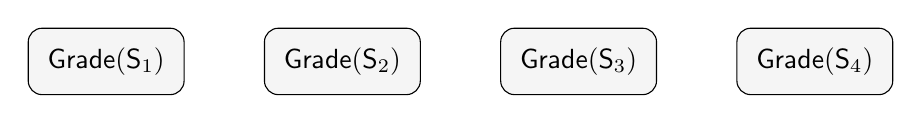
\begin{tikzpicture}
%			\node[dpadded,] (S) {$\var{Student}$};
			\foreach \i in {1,2,...,4} {
				\node[dpadded] (G1) at ($(3*\i,0)$) {$\var{Grade}(\var{S}_{\i})$};
			}
%			\draw[arr] (S) -- node[above]{$f$} (G);
			
		\end{tikzpicture}
    	
    	
        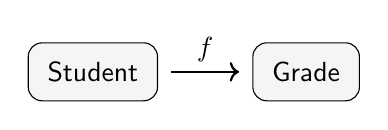
\begin{tikzpicture}
            \node[dpadded,] (S) {$\var{Student}$};
            \node[dpadded, right=of S] (G) {$\var{Grade}$};
            \draw[arr] (S) -- node[above]{$f$} (G);
            
        \end{tikzpicture}
    \end{center}    
\end{example}

A PDG need not be a collection of beliefs about the model itself, but rather beliefs about how the model looks, particularly from the angles that are easiest to represent. We do not need to actually have enough memory to describe a possible outcome, to reason about its properties.
For instance, a vector may have many more dimensions than it is possible for a human to store, but this fact need not prevent us from reasoning about the vector. Vector operations are described point-wise, which is why finite mathematicians are able to think about (at least some properties of) vector spaces with infinite dimensions. While it is true that doing so fails to capture many possibly relevant features of a giant vector, it allows us to reason with a smaller object, and gives us a set of possible worlds. 

From a technical standpoint, we are able to achieve the compression because the variables of the PDG heavily constrain the language of queries. While it may be the case that students in \Cref{ex:student}




The source of the confusion is the fact that 

\todo{
\section{The Deal With Uncertainty}

There are two ways to add probabilities here. One is to  

The addition of probability generally makes things substantially more complicated, but in our case it actually helps things up.


%\begin{minipage}{\textwidth}
\begin{center}
    \begin{tikzcd}[ampersand replacement=\&]
        %\Big\{\text{joints }\mu : \Delta(X \times Y) \Big\} 
        \Big\{\text{functions}~f : X \to Y\Big\} \& \Big\{\text{relations }R: X \times Y \to \mathbbm2\Big\} \\
        \Big\{\text{prob funcs }p : X \to \Delta Y \Big\} \& \Big\{\text{joints }\mu : \Delta(X \times Y) \Big\} \& 
         \Big\{\text{energies } E : X \times Y \to \mathbb R^+ \Big\} 
    \end{tikzcd}
\end{center}
%\end{minipage}

In the deterministic case, the distinction involves counter-factual information.

}

\section{Formal Correspondence: PDGs and Probabilistic Databases}

\subsection{The Deterministic Case}

\begin{defn}
	If $\mathbdcal{D} = (\mathcal D, I, a, \tau, \mathcal R)$ is a typed database, we construct its corresponding DG $\PDGof\D$ by 
	%	\begin{equation*}
	\[ 
	%		\left(
	\begin{array}{rlL}
		\PDGof{\mathbdcal D} := \Bigg(\quad	\N &:= \mathcal R \cup \mathcal D,
		& Nodes for both rows and columns \\[-0.5em]
		\Ed &:= \Big\{ \ed{R_i.\var A}{R_i}{\var A} \text{ where }\var A := \tau_{i,j}~\Big|~ i \in I, 1 \leq j \leq a_i \Big\},  
		&  Label with object path \\[0.5em]
		\V &:= 
		\begin{cases}
			R_i \mapsto R_i \\
			D \mapsto D
		\end{cases}~~, & Relation variables are rows \\[-0.7em]
		%			(R_i) &:= R_i = \{ (x_1, \ldots x_n) : (x_1, \ldots x_n) \in R_i \},  \\
		%			\V(D) &:= D,  \\
		\bp[R_i \to \var A] &:= (\ldots, x_{\var A}, \ldots) \mapsto \delta_{x_A}~~ \Bigg)
		& a point mass on the attribute
	\end{array} 
	\]
	%	\right)
	%	\end{equation*}
\end{defn}


\begin{defn}
	If $\pdgvars$ is a DDG, its corresponding probabilistic database is given by:
	
	\begin{equation*}
		content
	\end{equation*}
\end{defn}

\section{Relational Algebra: Database Operations on PDGs}
One can follow along with the \href{https://en.wikipedia.org/wiki/Relational_algebra}{wikipedia page} on relational algebra.

\begin{description}
\item[{Carteisan Product [\Cref{fig:cart}].}]
The Carteisan product is an operation that takes two variables $\var R_1$ and $\var R_2$, and produces a third variable $\var R_3$, such that has all outgoing arrows from both $\var R_1$ and $\var R_2.$  The tables are restricted so that they share no attributes, which here means that there is no variable that has both an arrow from $\var R_1$ and $\var R_2$.

The blue lines are the new ones created by the Cartesian product, which are generated by the two projections (dotted lines representing foreign keys, and not generally handled explicitly. However, they are the standard projections edges that we have been using in our discussion of PDGs, and their compositions with table attributes generate the solid blue arrows.

\item[{Unions and Intersections  [\Cref{fig:union+intersect}].}]
Unions and intersections are restricted to ``union compatible'' tables --- that is, tables that share the same sets of attributes. 
In the diagram below, the purple arrows are the those associated with the union, and are defined pointwise by the appropriate black arrow from $R_1$ or $R_2$ depending on the value. The blue arrows are those for the intersection, and can be equivalently defined by either black arrow, as $\V(\var R_1 \cap \var R_2)$ only contains those rows that are the same in $R_1$ and $R_2$.
\begin{figure}
	\begin{subfigure}{0.41\textwidth}
		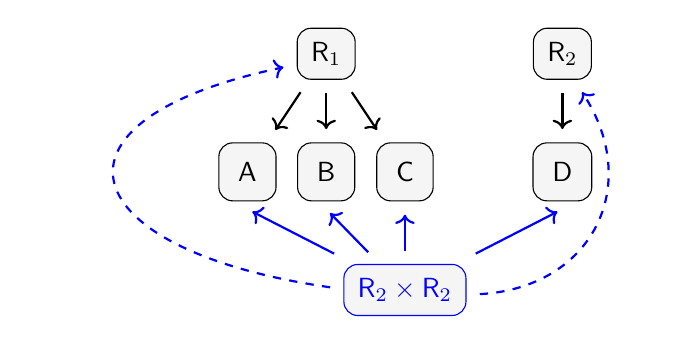
\begin{tikzpicture}
			\node[dpadded] (A) at (0,0){$\var A$};
			\node[dpadded] (B) at (1,0){$\var B$};
			\node[dpadded] (C) at (2,0){$\var C$};
			\node[dpadded] (D) at (4,0){$\var D$};
			
			\node[dpadded, inner sep=5pt] (R1) at (1,1.5){$\var R_1$};
			\node[dpadded, inner sep=5pt] (R2) at (4,1.5){$\var R_2$};
			
			\draw[arr] (R1) -- (A);
			\draw[arr] (R1) -- (B);
			\draw[arr] (R1) -- (C);
			\draw[arr] (R2) -- (D);
			
			\begin{scope}[blue]
				\node[dpadded, inner sep=5pt](R12) at (2,-1.5){$\var R_2 \times \var R_ 2$};
				\draw[arr] (R12) -- (A.south);
				\draw[arr] (R12) -- (B.south);
				\draw[arr] (R12) -- (C.south);
				\draw[arr] (R12) -- (D.south);
				
				\draw[arr, dashed] (R12) to[bend left=70, looseness=3, in=90] (R1);
				\draw[arr, dashed] (R12) to[bend right=60, looseness=1.3] (R2);
			\end{scope}
		\end{tikzpicture}
		\caption{Cartesian Product}\label{fig:cart}
	\end{subfigure}
	~~~~\hfill\vline\hfill
	\begin{subfigure}{0.51\textwidth}
	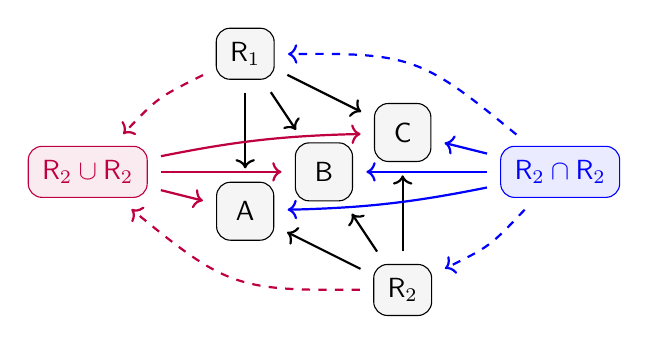
\begin{tikzpicture}
		\node[dpadded] (A) at (0,-0.5){$\var A$};
		\node[dpadded] (B) at (1,0){$\var B$};
		\node[dpadded] (C) at (2,0.5){$\var C$};
		
		\node[dpadded, inner sep=5pt] (R1) at (0,1.5){$\var R_1$};
		\node[dpadded, inner sep=5pt] (R2) at (2,-1.5){$\var R_2$};
		
		\draw[arr] (R1) -- (A);
		\draw[arr] (R1) -- (B);
		\draw[arr] (R1) -- (C);
		\draw[arr] (R2) -- (A);
		\draw[arr] (R2) -- (B);
		\draw[arr] (R2) -- (C);
		
		\begin{scope}[purple,dpadded/.append style={fill=purple}]
			\node[dpadded, inner sep=5pt](R12) at (-2,0){$\var R_2 \cup \var R_ 2$};
			\draw[arr] (R12) -- (A);
			\draw[arr] (R12) -- (B);
			\draw[arr] (R12) to [bend left=5] (C);
			
			
			\draw[arr, dashed] (R1) to[bend right=10, looseness=1.3] (R12);
			\draw[arr, dashed] (R2) to[bend left=20, looseness=1.3] (R12);
		\end{scope}
		\begin{scope}[blue,dpadded/.append style={fill=blue}]
			\node[dpadded, inner sep=5pt](R12) at (4,0){$\var R_2 \cap \var R_ 2$};
			\draw[arr] (R12) to [bend left=5] (A);
			\draw[arr] (R12) -- (B);
			\draw[arr] (R12) -- (C);
			
			\draw[arr, dashed] (R12) to[bend right=20, looseness=1.3] (R1);
			\draw[arr, dashed] (R12) to[bend left=10, looseness=1.3] (R2);
		\end{scope}
	\end{tikzpicture}
	\caption{Union and Intersection}\label{fig:union+intersect}
\end{subfigure}\\
	\caption{}
	\label{fig:cart+union+intersect}
\end{figure}
\begin{remark}
	The intersection and the Cartesian product are related extremes (for disjoint and identical attribute sets) of a single operation, which is a clear example of a \href{https://en.wikipedia.org/wiki/Limit_(category_theory)}{categorical limit} of the graph as a diagram of Sets.
	
	Intuitively, the limit of a diagram is a minimal object and set of maps from it to the diagram, that is compatible with the arrows already in the diagram (in that each arrow forms a commutative diagram with the new maps). 
\end{remark}

\item[{Projection  [\Cref{fig:project}].}]
Now come the three important main predicates of relational algebra, as given in \cite{Codd}.  The first is ``projection'', which given a table $\var R$ and attributes $\bf A$ returns a new table $\Pi_{\bf A}(\var R)$, whose columns are $\mat A$. 
\begin{figure*}
	\centering
	\begin{subfigure}{0.3\textwidth}
	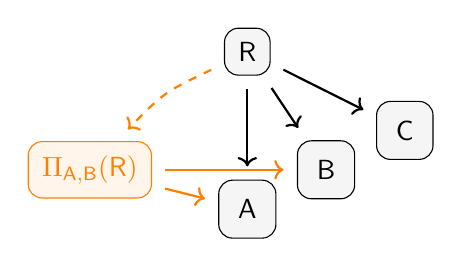
\begin{tikzpicture}
		\node[dpadded] (A) at (0,-0.5){$\var A$};
		\node[dpadded] (B) at (1,0){$\var B$};
		\node[dpadded] (C) at (2,0.5){$\var C$};
		
		\node[dpadded, inner sep=5pt] (R1) at (0,1.5){$\var R$};
		
		\draw[arr] (R1) -- (A);
		\draw[arr] (R1) -- (B);
		\draw[arr] (R1) -- (C);

		\begin{scope}[orange,dpadded/.append style={fill=orange}]
			\node[dpadded, inner sep=5pt](R12) at (-2,0){$\Pi_{\var{A,B}}(\var R)$};
			\draw[arr] (R12) -- (A);
			\draw[arr] (R12) -- (B);
%			\draw[arr] (R12) to [bend left=5] (C);
					
			\draw[arr, dashed] (R1) to[bend right=10, looseness=1.3] (R12);

		\end{scope}
	\end{tikzpicture}
\caption{Projection}\label{fig:project}
	\end{subfigure}
	\hfill\vline\hfill
	\begin{subfigure}{0.29\textwidth}
	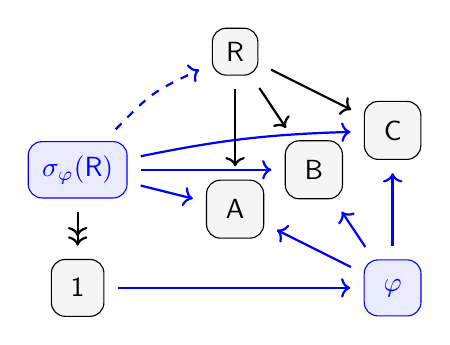
\begin{tikzpicture}%[scale=0.85]
		\node[dpadded] (A) at (0,-0.5){$\var A$};
		\node[dpadded] (B) at (1,0){$\var B$};
		\node[dpadded] (C) at (2,0.5){$\var C$};
		\node[dpadded] (1) at (-2, -1.5){$\var 1$};
		
		\node[dpadded, inner sep=5pt] (R1) at (0,1.5){$\var R$};
		
		\draw[arr] (R1) -- (A);
		\draw[arr] (R1) -- (B);
		\draw[arr] (R1) -- (C);
		
		\begin{scope}[blue,dpadded/.append style={fill=blue}]
			\node[dpadded, inner sep=5pt](R12) at (-2,0){$\sigma_\varphi(\var R)$};
			\node[dpadded] (phi) at (2, -1.5){$\var\varphi$};
			%			\coordinate (Q) at (barycentric cs:phi=3,A=1,B=1,C=1);
			%			\begin{scope}[shorten <=0, shorten >=0]
			%				\draw[arr, -] (Q) -- (A) (Q) -- (C) (B) -- (Q);
			%			\end{scope}
			%			\draw[arr, shorten <=0] (Q) -- (phi);
			\draw[arr] (phi) -- (A);
			\draw[arr] (phi) -- (B);
			\draw[arr] (phi) -- (C);
			\draw[arr] (1) -- (phi);
			\draw[arr, thick] (R12) -- (A);
			\draw[arr, thick] (R12) -- (B);
			\draw[arr] (R12) to [bend left=5] (C);
			
			\draw[arr, dashed] (R12) to[bend left=10, looseness=1.3] (R1);
			
		\end{scope}
		\draw[arr,->>] (R12) -- (1);
	\end{tikzpicture}
\caption{Selection}\label{fig:selection}
	\end{subfigure}
	\hfill\vline\hfill
\begin{subfigure}{0.3\textwidth}
		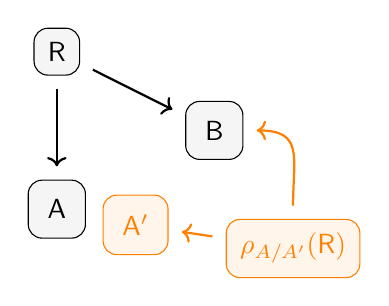
\begin{tikzpicture}
		\node[dpadded] (A) at (0,-0.5){$\var A$};
		
		\node[dpadded] (B) at (2,0.5){$\var B$};
		
		\node[dpadded, inner sep=5pt] (R1) at (0,1.5){$\var R$};
		
		\draw[arr] (R1) -- (A);
		\draw[arr] (R1) -- (B);
		
		\begin{scope}[orange,dpadded/.append style={fill=orange}]
			\node[dpadded, inner sep=5pt](R12) at (3,-1){$\rho_{A/A'}(\var R)$};
			%		\draw[arr] (R1) -- (A');
			\node[dpadded] (A') at (1,-0.7){$\var A'$};
			\draw[arr] (R12) -- (A');
			%			\draw[arr] (R12) -- (B);
			\draw[arr] (R12) to [in=0, out=90, looseness=1.5] (B);
			%			\draw[arr, dashed] (R12) to[bend left=10, looseness=1.3] (R1);
		\end{scope}
	\end{tikzpicture}
\caption{Rename}\label{fig:rename}
\end{subfigure}
\caption{}
\end{figure*}
In relational algebra, the index row of the new column may be smaller, if some rows of $\var R$ cannot be distinguished by the selected projection columns, but in SQL this is not the case unless one employs the \texttt{DISTINCT} keyword.

\item[{Selection [\Cref{fig:selection}].}]
Selection too is a limit; it consists of those rows that satisfy the predicate $\varphi$. 
It can be implemented by other operations also; as a relation, it is the intersection /natural join of $\var R$ with $\varphi$ thought of as a relation, containing all tuples $\alpha$ for which $\varphi(\alpha)$ is true. Alternatively, it can be viewed as the limit of the diagram below, which can be read as (1) an inclusion of $\varphi$ into the diagram as a table itself, and (2) an assertion that it is true.

\item[{Rename [\Cref{fig:rename}].}]
Finally, to emulate $\rho_{A/A'}(\var R)$, copy $\var R$ and $A$; call the copied variable $\var A'$, and give $\rho_{A/A'}(\var R)$ the arrows as $\var R$, except replace the one from $\var R$ to $\var A$ with an identical one from $\var R$ to $\var A'$. 




\item[{Natural Join [\Cref{fig:natjoin}]}]

Therefore the natural join is the fiber product, or pullback, of the commuting square, and is the generalization of the intersection and cartesian product.

The example below differs from the illustration of a Cartesian product only in that it includes $\var B$ as an attribute of $\var R_2$ in addition to $\var R_1$. Therefore, the pullback has to equalize this structure, and so $\var R_1 \bowtie \var R_2$ has only those rows for which the ultra bold arrows give the same value of $\var B$. 
\begin{figure}
	\centering
	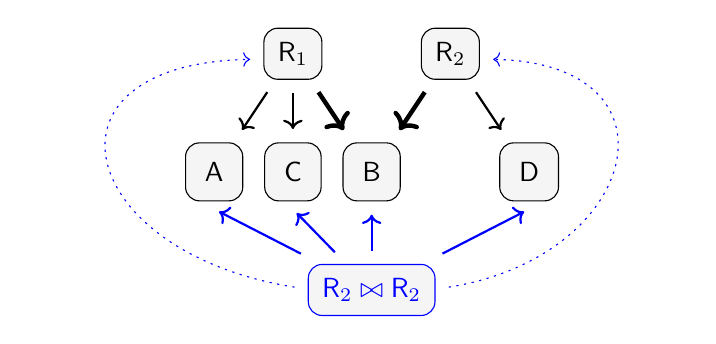
\begin{tikzpicture}
	\node[dpadded] (A) at (0,0){$\var A$};
	\node[dpadded] (B) at (2,0){$\var B$};
	\node[dpadded] (C) at (1,0){$\var C$};
	\node[dpadded] (D) at (4,0){$\var D$};
	
	\node[dpadded, inner sep=5pt] (R1) at (1,1.5){$\var R_1$};
	\node[dpadded, inner sep=5pt] (R2) at (3,1.5){$\var R_2$};
	
	\draw[arr] (R1) -- (A);
	\draw[arr, ultra thick] (R1) -- (B);
	\draw[arr] (R1) -- (C);
	\draw[arr] (R2) -- (D);
	\draw[arr, ultra thick] (R2) -- (B);
	
	\begin{scope}[blue]
		\node[dpadded, inner sep=5pt](R12) at (2,-1.5){$\var R_2 \bowtie \var R_ 2$};
		\draw[arr] (R12) -- (A.south);
		\draw[arr] (R12) -- (B.south);
		\draw[arr] (R12) -- (C.south);
		\draw[arr] (R12) -- (D.south);
		
		\draw[arr, dotted, thin] (R12) to[bend left=70, looseness=2.5, in=80] (R1);
		\draw[arr, dotted, thin] (R12) to[bend right=70, looseness=2.2, in=-80] (R2);
	\end{scope}
\end{tikzpicture}
\caption{Diagram of the natural join. The two bold arrows are asserted to represent the same variable.}\label{fig:natjoin}
\end{figure}
\end{description}
%\todo

\section{Link Guard Variables} \label{sec:link-gurad}

Often predicates are false, when we talk about them, we do not want to assert their truth. 
Without any modifications, a link $\ed LXY$ in a PDG $\dg M$ is effectively an assertion that the variables $X$ and $Y$ enjoy the relation described by $L$. Interpreted in the relational setting, we have specified a (directed and probabilistic) relation $L$, between $X$ and $Y$; but it may be that this relation does not hold. At the very least, we might want to entertain the possibility.%
	\footnote{Entertaining this possibility means we are no longer quite using an \emph{optimal} encoding to transmit our beliefs, but rather also adding some additional bits of redundancy to make sure that. This appears to be analogous to a noisy channel in information theory.}

\section{The Computation of a PDG} \label{sec:automaton}
The scoring semantics $\bbr{-}$ developed in the previous work is clearly only enough to capture the joint-distribution view of a possible world. However, given that scoring functions are contravariant, we may as well extend it to other, more general general objects. At the same time, we will be able to explain how PDGs can be computed with. 






\todo{But when these more general objects marginalize to joint distributions, either we lose coherence, or...?
Given that the scoring function for joint distributions don't quite capture all notions of possible worlds.
The original PDG semantics (the score of a joint distribution) may now be recovered as a 
}



\bibliographystyle{alpha}
\bibliography{../papers/repr/joe.bib,../db.bib}
\appendix

    
\end{document}
